\documentclass{article}

\usepackage[english]{babel}
\usepackage[utf8]{inputenc}
\usepackage{amsmath,amssymb}
\usepackage{parskip}
\usepackage{graphicx}
\usepackage{listings}
\usepackage{subfig}
\usepackage{float}
\lstset{
    numbers=left, 
    numberstyle= \tiny, 
    keywordstyle= \color{ blue!70},
    commentstyle= \color{red!50!green!50!blue!50}, 
    frame=shadowbox, % 阴影效果
    rulesepcolor= \color{ red!20!green!20!blue!20} ,
    escapeinside=``, % 英文分号中可写入中文
    xleftmargin=2em,xrightmargin=2em, aboveskip=1em,
    framexleftmargin=2em,
    breaklines=true,
    language=R
} 

% Margins
\usepackage[top=2.5cm, left=3cm, right=3cm, bottom=4.0cm]{geometry}
% Colour table cells
\usepackage[table]{xcolor}

% Get larger line spacing in table
\newcommand{\tablespace}{\\[1.25mm]}
\newcommand\Tstrut{\rule{0pt}{2.6ex}}         % = `top' strut
\newcommand\tstrut{\rule{0pt}{2.0ex}}         % = `top' strut
\newcommand\Bstrut{\rule[-0.9ex]{0pt}{0pt}}   % = `bottom' strut

%%%%%%%%%%%%%%%%%
%     Title     %
%%%%%%%%%%%%%%%%%
\title{CSCI946 Assignment}
\author{Yao Xiao \\ SID 2019180015}
\date{\today}

\begin{document}
\maketitle

%%%%%%%%%%%%%%%%%
%   Problem 1   %
%%%%%%%%%%%%%%%%%
\section{Task One}
\begin{lstlisting}
library("rpart")
library("rpart.plot")

dtrain = read.table("DTdata.csv",header = TRUE,sep=",")
dtrain

# make a simple decision tree
fit = rpart(Play ~ Outlook + Temperature + Humidity + Wind,method = "class",
            data = dtrain,
            control = rpart.control(minsplit = 1),
            parms = list(split='information'))

summary(fit)

# plot the tree
rpart.plot(fit,type=4,extra=1)

# create the new observation
obs = data.frame(Outlook="rainy",Temperature="hot",Humidity="high",Wind=TRUE)

#prediction outcome for a new observation
predict(fit,obs=obs,type="prob")

\end{lstlisting}


\begin{figure}[H]
    \subfloat{
        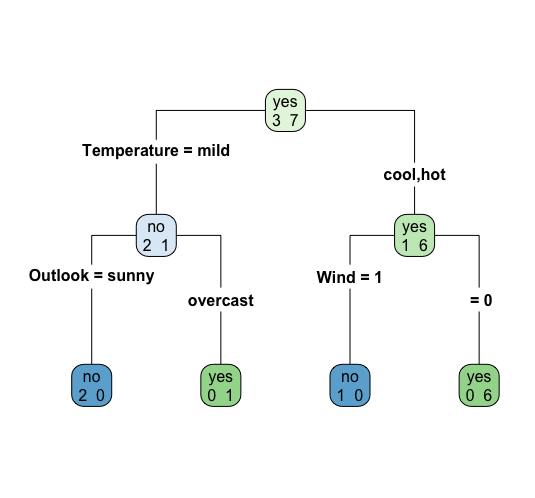
\includegraphics[width=0.9\textwidth]{Fig1}
    }\\
    \subfloat{
        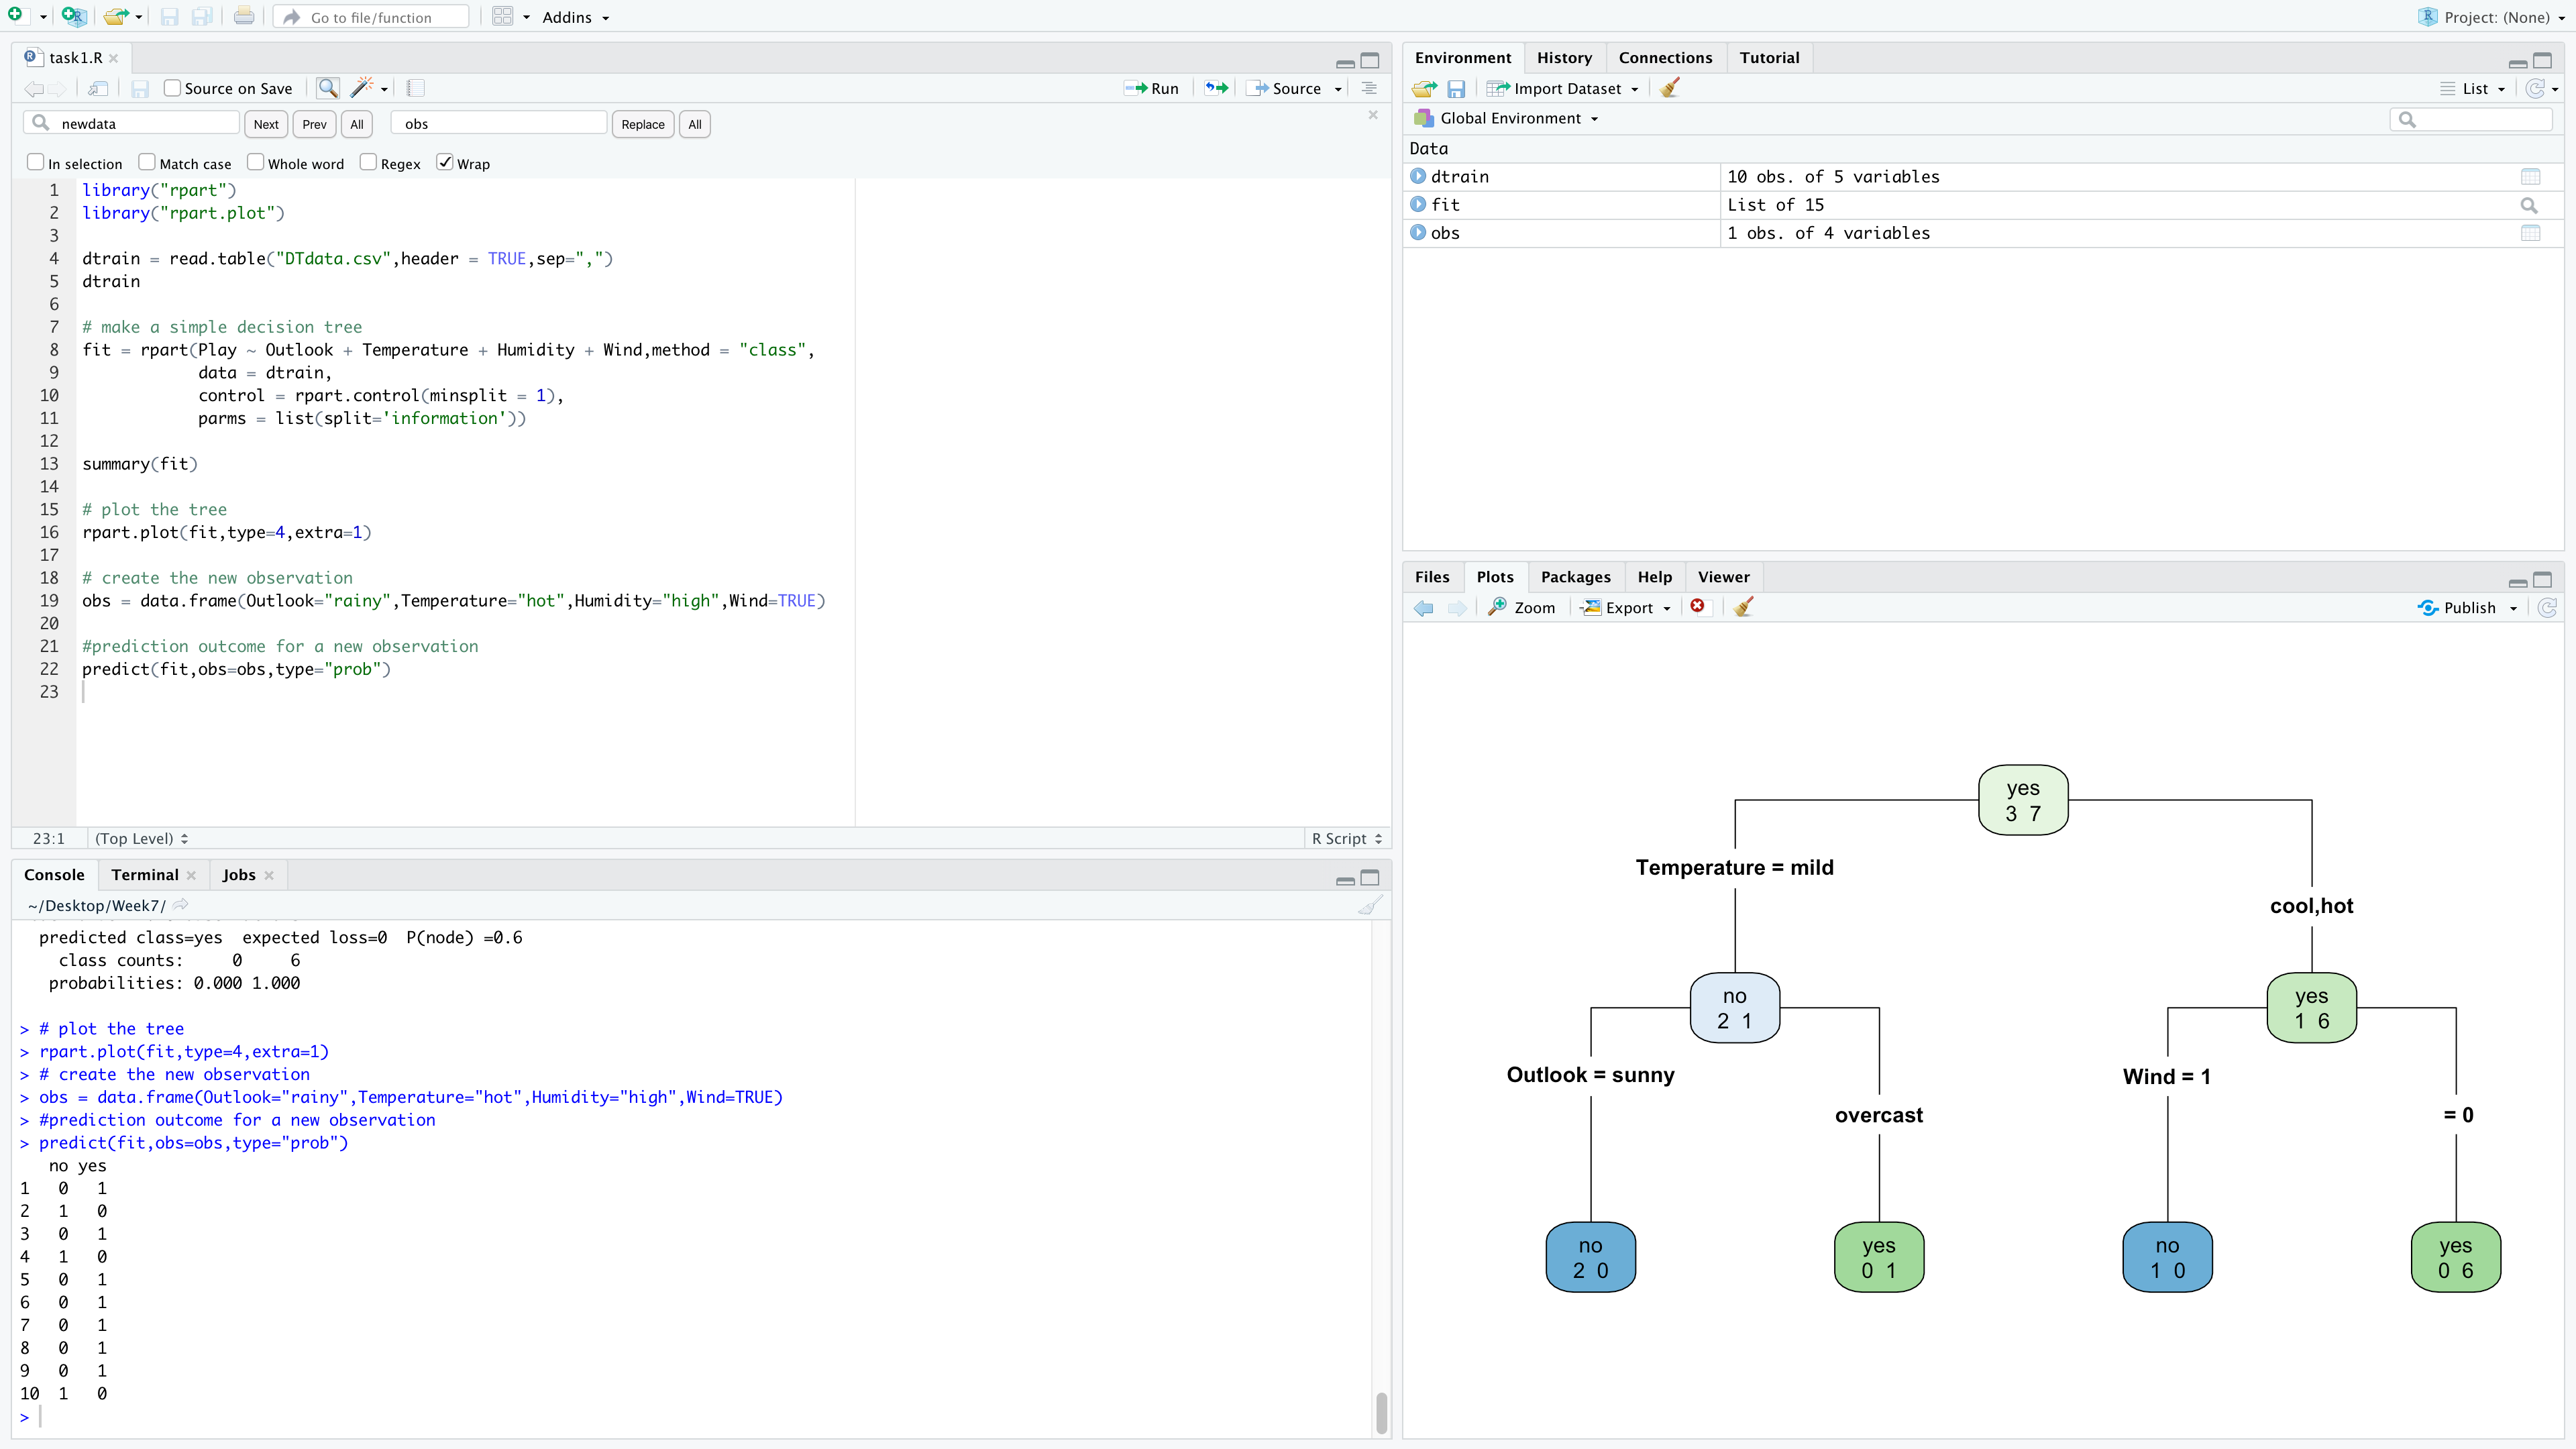
\includegraphics[width=0.9\textwidth]{Fig2}
    }
\end{figure}


\section{Task Two}
\begin{lstlisting}
library("e1071")

df = read.table("sample1.csv",header = TRUE,sep = ",")
df

traindata = as.data.frame(df[1:14,])
traindata
testdata = as.data.frame(df[15,])
testdata

# build model
model = naiveBayes(Enrolls ~ Age+Income+JobSatisfaction+Desire,traindata,laplace = 0.01)
model

# make the prediction
results = predict(model, newdata = testdata, type = "raw")
results

\end{lstlisting}

\begin{figure}[H]
    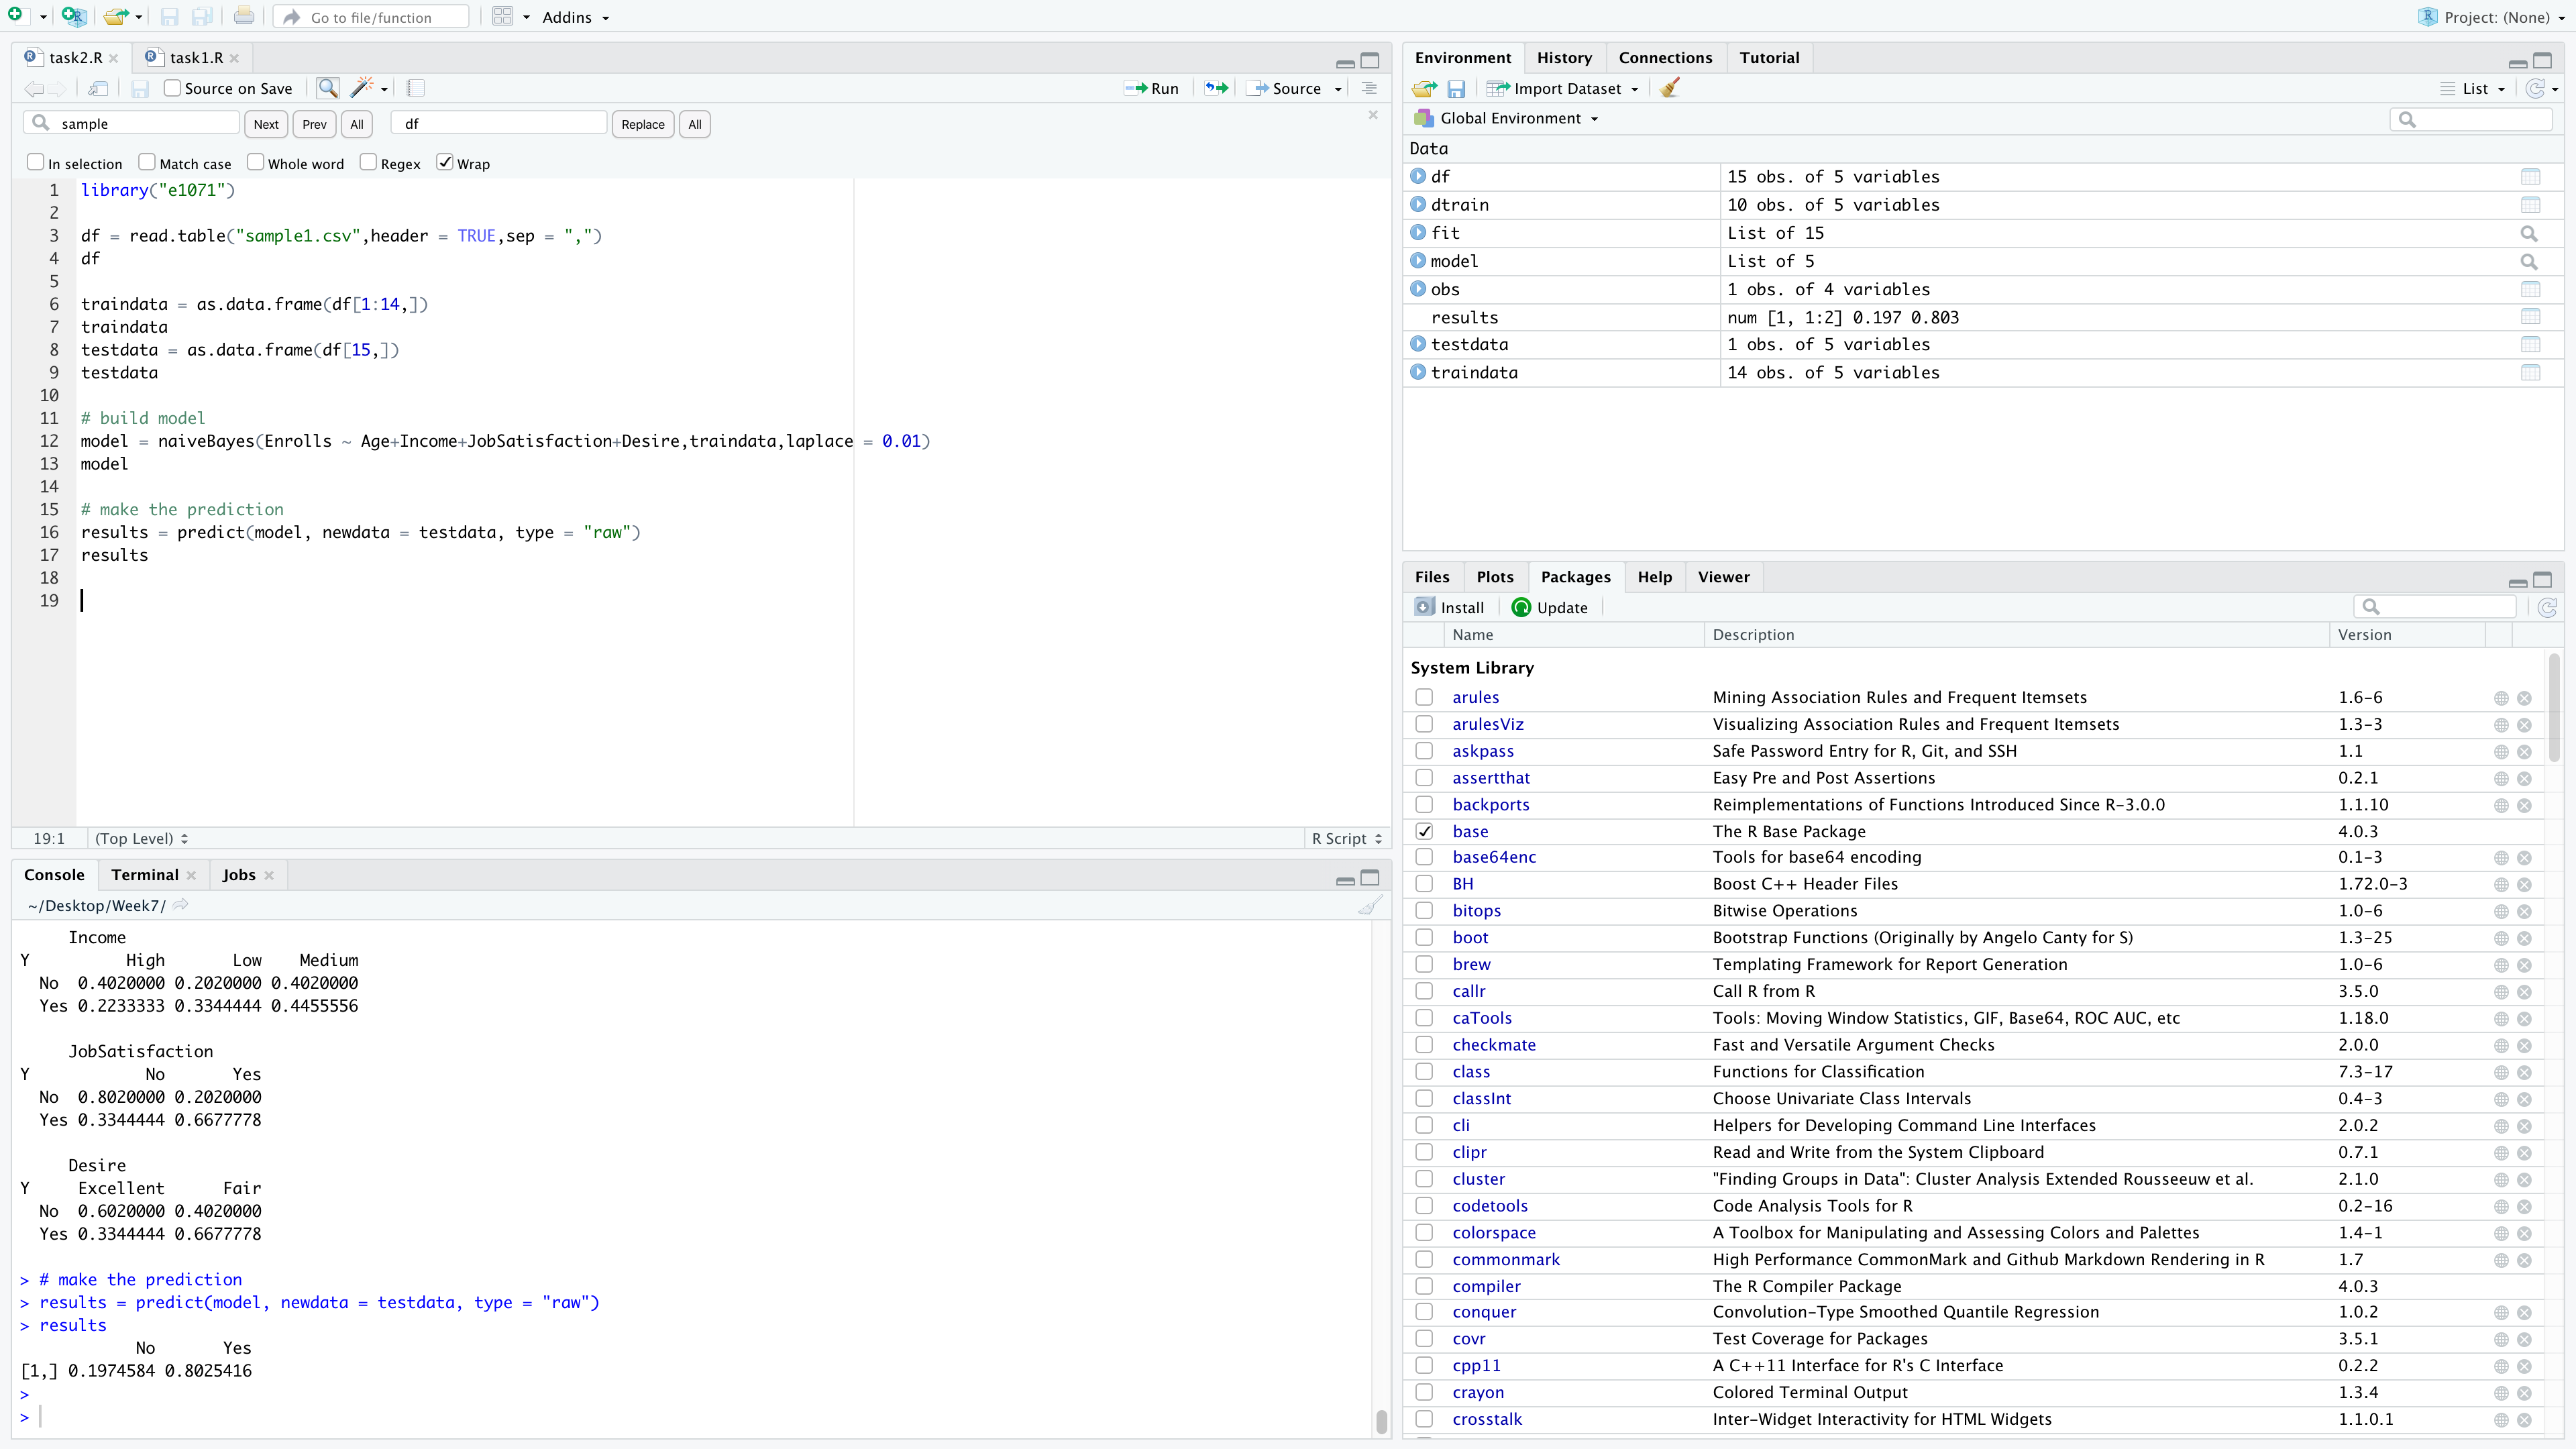
\includegraphics[width=0.9\textwidth]{Fig3}
\end{figure}


\end{document}
